\documentclass[oneside]{book}
\usepackage{glossaries}
\usepackage{derivative}
\usepackage{pgfplots}
\usepackage{graphicx}
\usepackage{tikz}
\usepackage{float}
\usepackage{lipsum}
\usepackage{circuitikz}
\usepackage{amsmath}
\usepackage{fancyhdr}
\usepackage{amssymb}
\usepackage{subcaption}
\usepackage{lastpage}
\usepackage{array}
\usepackage[a4paper,
    left=10mm,
    right=10mm,
    top=12mm,
    bottom=12mm,
]{geometry}
\setcounter{tocdepth}{3}
\newcolumntype{P}[1]{>{\centering\arraybackslash}p{#1}}
\begin{document}
\pagestyle{fancy}
    \fancyhf{}
\fancyhead[L]{EGB120 Foundations of Electrical Engineering}
\fancyhead[R]{\nouppercase{\leftmark}}
\fancyfoot[L]{Dinal Atapattu}
\renewcommand{\footrulewidth}{0.4pt}
\fancyfoot[R]{Page \thepage\ of \pageref{LastPage}}
    \title{
            Queensland University of Technology\\
            \rule{\linewidth}{0.5pt}
        \centering
        \textbf{EGB120} \\
        Foundations of Electrical Engineering\\
        \vspace{0.4cm}
        \rule{\linewidth}{1.5pt}
        \small{\textit{Profressor Geoff Walker}}
    }
    \author{Dinal Atapattu}
    \date{\today}
    \maketitle
    \thispagestyle{empty}
    \tableofcontents
        \chapter{Electrical Circuits}
            \section{Fundamental Units}
                \begin{figure}[H]
                    \centering
                    \begin{tabular}{|p{0.15\textwidth}|p{0.4\textwidth}|p{0.15\textwidth}|p{0.15\textwidth}|}
                        \hline
                        \textbf{Quantity} & \textbf{Definition} & \textbf{Symbol} & \textbf{SI Unit} \\
                        \hline
                        Charge & Physical property of matter that causes it to experience a force
                        when placed in an electromagnetic field & $q$ & Coulomb (C) \\
                        \hline
                        Current & \begin{equation*}i(t) = \odv{q}{t}\end{equation*} & $i$ & Ampere (A) \\
                        \hline
                        Voltage & \begin{equation*}v(t) = \odv{w}{q}\end{equation*} & $v$ & Volt (V) \\
                        \hline
                        Power & \begin{equation*}p(t) = \odv{w}{t} = \odv{q}{t} \times \odv{w}{q} = vi \end{equation*} & $p$ & Watt (W) \\
                        \hline
                        Energy & \begin{equation*}w(\tau) = \int_{\tau}^{0} p(t) dt\end{equation*} & $e$ & Joule (J) \\
                        \hline
                    \end{tabular}
                \end{figure}
            \section{Basic Circuit Elements}
                \subsection{Voltage Source}
                    Produces or dissipates power at a specific voltage with whatever current is required
                \subsection{Current Source}
                    Produces or dissipates power at a specific current with whatever voltage is required
                \subsection{Resistor}
                    Dissipates power so that the voltage across the terminals is proportional to the current
                    \begin{align*}
                        v = Ri \tag{Ohm's Law}
                        \intertext{Following this}
                        p = vi = Ri^2 = \frac{v^2}{R}
                    \end{align*}
        \chapter{Simple Circuits}
            \section{Physics Ignored}
                \begin{itemize}
                    \item Electrical effects are instantaneous
                    \item Net charge on every component is zero
                    \item No magnetic coupling between components
                \end{itemize}
            \section{Series}
                Elements are connected end to end and \textbf{have the same current flowing through them}
                \begin{figure}[H]
                    \centering
                    \begin{circuitikz}
                        \draw (0,0) to[R=$R_1$] (2,0) to[R=$R_2$] (4,0) to[R=$R_3$] (6,0);
                    \end{circuitikz}
                    \caption{Series Circuit}
                \end{figure}
            \section{Parallel}
                Both ends of one element are connected directly and \textbf{have the same voltage across them}
                \begin{figure}[H]
                    \centering
                    \begin{circuitikz}
                        \draw (0,0) to[R=$R_1$] (0,2);
                        \draw (2,0) to[R=$R_2$] (2,2);
                        \draw (4,0) to[R=$R_3$] (4,2);
                        \draw (6,0) to[R=$R_4$] (6,2);
                        \draw (0,2) -- (6,2);
                        \draw (0,0) -- (6,0);
                    \end{circuitikz}
                    \caption{Parallel Circuit}
                \end{figure}
            \section{Kirchoff's Laws}
                \subsection{Kirchoff's Current Law}
                    The sum of currents entering a node is equal to the sum of currents leaving a node\\
                    \begin{minipage}{0.5\textwidth}
                        \begin{equation*}
                            \sum_{k=1}^{n} i_k = 0
                        \end{equation*}
                    \end{minipage}
                    \begin{minipage}{0.5\textwidth}
                        \begin{figure}[H]
                            \centering
                            \begin{circuitikz}
                                \draw (0,0) to[short, i=$i_1$] (2,0);
                                \draw (2,-2) to[short, i=$i_2$] (2,0);
                                \draw (4,0) to[short, i=$i_3$] (2,0);
                                \node at (2,0.7) {$i_1 + i_2 + i_3 = 0$};
                            \end{circuitikz}
                            \caption{Kirchoff's Current Law}
                        \end{figure}
                    \end{minipage}
                \subsection{Kirchoff's Voltage Law}
                    The sum of voltages around a closed loop is zero\\
                    \begin{minipage}{0.5\textwidth}
                        \begin{equation*}
                            \sum_{k=1}^{n} v_k = 0
                        \end{equation*}
                    \end{minipage}
                    \begin{minipage}{0.5\textwidth}
                        \begin{figure}[H]
                            \centering
                            \begin{circuitikz}[american]
                                \draw (0,2) to[battery, v_=$v_1$] (0,0);
                                \draw (0,2) to[short] (2,2);
                                \draw (2,2) to[resistor, l_=$R_1$, v^=$v_2$] (2,0);
                                \draw (2,0) to[resistor, l_=$R_2$, v^=$v_3$] (0,0);
                            \end{circuitikz}
                            \begin{align*}
                                v_1 - v_2 - v_3 &= 0\\
                                v_1 &= v_2 + v_3
                            \end{align*}
                            \caption{Kirchoff's Voltage Law}
                        \end{figure}
                    \end{minipage}
            \section{Component Behaviours in Series and Parallel}
                \begin{figure}[H]
                    \centering
                    \begin{tabular}{p{0.15\textwidth} p{0.25\textwidth} p{0.25\textwidth}}
                        \hline
                        \textbf{Component} & \textbf{Series} & \textbf{Parallel} \\
                        \hline
                        Voltage Source & $v_s = v_1 + v_2 + v_3$ & $v_s = v_1 = v_2 = v_3$\\
                        \hspace{0.2cm}\\
                        Current Source & $i_s = i_1 = i_2 = i_3$ & $i_s = i_1 + i_2 + i_3$\\
                        \hspace{0.2cm}\\
                        Resistor & $R_s = R_1 + R_2 + R_3$ & $\frac{1}{R_s} = \frac{1}{R_1} + \frac{1}{R_2} + \frac{1}{R_3}$\\
                        \hspace{0.2cm}\\
                        Inductor & $L_s = L_1 + L_2 + L_3$ & $\frac{1}{L_s} = \frac{1}{L_1} + \frac{1}{L_2} + \frac{1}{L_3}$\\
                        \hspace{0.2cm}\\
                        Capacitor & $\frac{1}{C_s} = \frac{1}{C_1} + \frac{1}{C_2} + \frac{1}{C_3}$ & $C_s = C_1 + C_2 + C_3$\\
                        \hspace{0.2cm}\\
                        \hline
                    \end{tabular}
                    \caption{Component Behaviours in Series and Parallel}
                \end{figure}
            \section{Voltage Divider}
                \begin{minipage}{0.6\linewidth}
                    \begin{figure}[H]
                        \centering
                        \begin{circuitikz}[american]
                            \draw (0,0) to[battery, v_=$v_s$, invert] (0,4);
                            \draw (0,4) to[short] (2,4);
                            \draw (2,4) to[resistor, l_=$R_1$, v^=$v_1$] (2,2);
                            \draw (2,2) to[resistor, l_=$R_2$, v^=$v_2$] (2,0);
                            \draw (2,0) to[short] (0,0);
                            \draw (2,2) to[short] (4,2); 
                            \draw (2,0) to[short] (4,0); 
                        \end{circuitikz}
                        \caption{Voltage Divider}
                    \end{figure} 
                \end{minipage}
                \begin{minipage}{0.3\linewidth}
                    \begin{flalign*}
                        \intertext{Current through resistors is}
                        i &= \frac{v_s}{R_1 + R_2}\\
                        \intertext{Voltage across resistors is}
                        v_1 &= iR_1 = \frac{R_1}{R_1 + R_2}v_s\\
                        \intertext{For more resistors}
                        v_k &= \frac{R_j}{R_{eq}}v_s
                    \end{flalign*}
                \end{minipage}
            \section{Current Divider}
                \begin{minipage}{0.6\linewidth}
                    \begin{figure}[H]
                        \centering
                        \begin{circuitikz}[american]
                            \draw (0,0) to[current source, v^=$i$] (0,2);
                            \draw (2,2) to[resistor, l_=$R_1$, i^=$i_1$] (2,0);
                            \draw (4,2) to[resistor, l_=$R_2$, i^=$i_2$] (4,0);
                            \draw (6,2) to[resistor, l_=$R_3$, i^=$i_3$] (6,0);
                            \draw (0,0) to[short] (6,0);
                            \draw (0,2) to[short] (6,2);
                        \end{circuitikz}
                        \caption{Current Divider}
                    \end{figure} 
                \end{minipage}
                \begin{minipage}{0.3\linewidth}
                    \begin{flalign*}
                        \intertext{Voltage across resistors is}
                        v &= i(R_1 || R_2 || R_3)\\
                        \intertext{Current through resistors is}
                        i_j &= \frac{v}{R_j} = \frac{R_1 || R_2 || R_3}{R_j}i\\
                        \intertext{For more resistors}
                        i_j &= \frac{R_{eq}}{R_{j}}i
                    \end{flalign*}
                \end{minipage}
        \chapter{Diodes}
            Current flows from the anode to the cathode and the voltage across the diode is positive.\\
            A diode requires voltage to be applied across it to conduct current. This voltage is called the \textbf{forward voltage}.
            \section{Voltage-Current Characteristics}
                \begin{figure}[htbp]
                    \centering
                    \begin{subfigure}{0.3\textwidth}
                        \centering
                        \begin{tikzpicture}
                            \begin{axis}[
                                xlabel={Voltage (V)},
                                ylabel={Current (A)},
                                title={Resistor},
                                width=\linewidth,
                                height=\linewidth,
                                xmin=-1, xmax=11,
                                ymin=-1, ymax=11,
                                xtick={0, 5, 10},
                                ytick={0, 5, 10},
                            ]
                            \addplot[domain=0:10, samples=100, color=red]{x};
                            \end{axis}
                        \end{tikzpicture}
                    \end{subfigure}
                    \begin{subfigure}{0.3\textwidth}
                        \centering
                        \begin{tikzpicture}
                            \begin{axis}[
                                xlabel={Voltage (V)},
                                ylabel={Current (A)},
                                title={Voltage Source},
                                width=\linewidth,
                                height=\linewidth,
                                xmin=-1, xmax=11,
                                ymin=-1, ymax=11,
                                xtick={0, 5, 10},
                                ytick={0, 5, 10},
                            ]
                            \addplot[domain=0:10, samples=100, color=red] coordinates {
                                (7, 0)
                                (7, 10)
                            };
                            \end{axis}
                        \end{tikzpicture}
                    \end{subfigure}
                    \begin{subfigure}{0.3\textwidth}
                        \centering
                        \begin{tikzpicture}
                            \begin{axis}[
                                xlabel={Voltage (V)},
                                ylabel={Current (A)},
                                title={Voltage Source},
                                width=\linewidth,
                                height=\linewidth,
                                xmin=-1, xmax=11,
                                ymin=-1, ymax=11,
                                xtick={0, 5, 10},
                                ytick={0, 5, 10},
                            ]
                            \addplot[domain=0:10, samples=100, color=red] coordinates {
                                (0, 7)
                                (10, 7)
                            };
                            \end{axis}
                        \end{tikzpicture}
                    \end{subfigure}
                    \caption{Diode VI Characteristics}
                \end{figure}
                \subsection{Simplified Diode Characteristics}
                    Diodes have non-linear characteristics. Therefore, they are simplified to make calculations easier.
                    \begin{figure}[H]
                        \centering
                        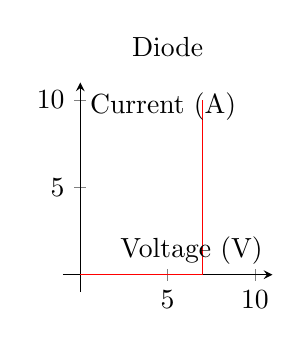
\begin{tikzpicture}
                            \begin{axis}[
                                xlabel={Voltage (V)},
                                ylabel={Current (A)},
                                title={Diode},
                                width=0.35\linewidth,  % Adjust the width to make the graph smaller
                                height=0.35\linewidth, % Adjust the height to make the graph smaller
                                xmin=-1, xmax=11,
                                ymin=-1, ymax=11,
                                xtick={0, 5, 10},
                                ytick={0, 5, 10},
                                axis lines=middle,   % Add x and y-axis lines
                            ]
                            \addplot[domain=0:10, samples=100, color=red] coordinates {
                                (0, 0)
                                (7, 0)
                                (7, 10)
                            };
                            \end{axis}
                        \end{tikzpicture}                        
                        \caption{Simplified Diode Characteristics}
                    \end{figure}
                \subsection{Full Diode Characteristics}
                    Diodes can be accurately modelled using Shcokley's equation
                    \begin{align*}
                        i_D = I_s \left( e^{\frac{v_D}{V_T} -1} \right) && V_T = \frac{kT}{q}
                    \end{align*}
                    where $I_s$ is the saturation current, $V_T$ is the thermal voltage, $k$ is Boltzmann's constant, $T$ is the temperature in Kelvin and $q$ is the charge of an electron.
            \section{Operating Points}
            \section{Load Lines}
        \chapter{Filters and Rectifiers}
            Filters keep the desired frequency components of a signal and remove the unwanted frequency components.\\
            They do this in the frequency domain
            \section{Applications of Filters}
                \begin{itemize}
                    \item Audio Signals
                    \begin{itemize}
                        \item Remove high frequency hiss (magnetic tape)
                        \item Remove low frequency rumble (vinyl)
                    \end{itemize}
                    \item Medical Signals
                    \begin{itemize}
                        \item EEG alpha waves are 8-12Hz
                        \item EEG beta waves are 12-30Hz
                        \item ECG waves are 1 - 40Hz
                    \end{itemize}
                    \item 50Hz interference
                    \begin{itemize}
                        \item Remove all signals near 50Hz
                    \end{itemize}
                    \item Signal Processing
                \end{itemize}
            \section{Ideal Filters}
                \begin{figure}[H]
                    \centering
                    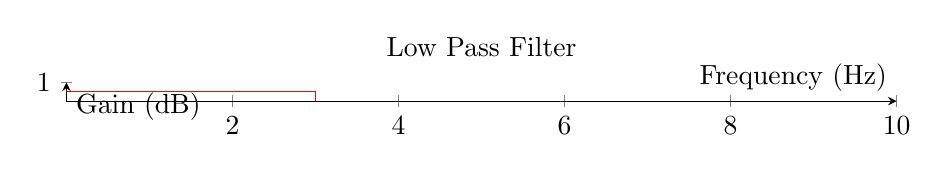
\begin{tikzpicture}
    \begin{axis}[
        xlabel={Frequency (Hz)},
        ylabel={Gain (dB)},
        title={Low Pass Filter},
        width=\linewidth,
        height=0.15\linewidth,
        xmin=0, xmax=10,
        ymin=0, ymax=1,
        ytick={1},
        xtick={0, 2, 4, 6, 8, 10},
        axis lines=middle,
    ]
    \addplot[domain=0:10, samples=100, color=red] coordinates {
        (0, 0.5)
        (3, 0.5)
        (3, 0)
    };
    \end{axis}
\end{tikzpicture}
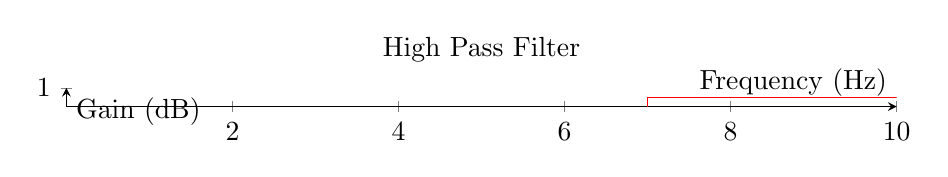
\begin{tikzpicture}
    \begin{axis}[
        xlabel={Frequency (Hz)},
        ylabel={Gain (dB)},
        title={High Pass Filter},
        width=\linewidth,
        height=0.15\linewidth,
        xmin=0, xmax=10,
        ymin=0, ymax=1,
        ytick={1},
        xtick={0, 2, 4, 6, 8, 10},
        axis lines=middle,
    ]
    \addplot[domain=0:10, samples=100, color=red] coordinates {
        (7, 0)
        (7, 0.5)
        (10, 0.5)
    };
    \end{axis}
\end{tikzpicture}
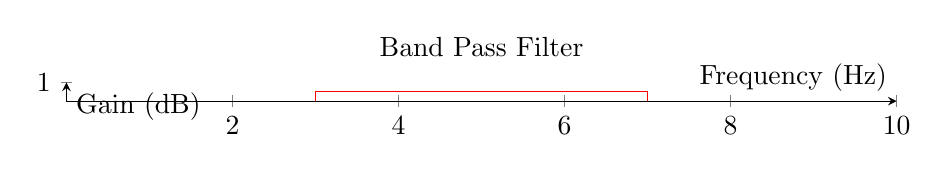
\begin{tikzpicture}
    \begin{axis}[
        xlabel={Frequency (Hz)},
        ylabel={Gain (dB)},
        title={Band Pass Filter},
        width=\linewidth,
        height=0.15\linewidth,
        xmin=0, xmax=10,
        ymin=0, ymax=1,
        ytick={1},
        xtick={0, 2, 4, 6, 8, 10},
        axis lines=middle,
    ]
    \addplot[domain=0:10, samples=100, color=red] coordinates {
        (3, 0)
        (3, 0.5)
        (7, 0.5)
        (7, 0)
    };
    \end{axis}
\end{tikzpicture}
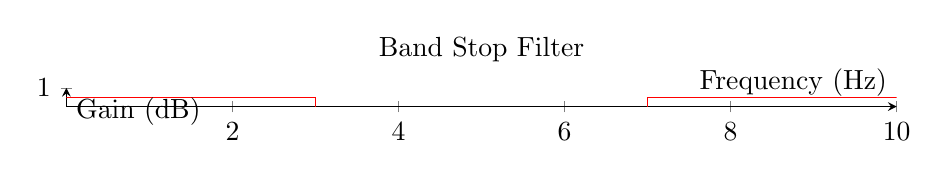
\begin{tikzpicture}
    \begin{axis}[
        xlabel={Frequency (Hz)},
        ylabel={Gain (dB)},
        title={Band Stop Filter},
        width=\linewidth,
        height=0.15\linewidth,
        xmin=0, xmax=10,
        ymin=0, ymax=1,
        ytick={1},
        xtick={0, 2, 4, 6, 8, 10},
        axis lines=middle,
    ]
     \addplot[domain=0:10, samples=100, color=red] coordinates {
        (0, 0.5)
        (3, 0.5)
        (3, 0)
    };
    \addplot[domain=0:10, samples=100, color=red] coordinates {
        (7, 0)
        (7, 0.5)
        (10, 0.5)
    };
    \end{axis}
\end{tikzpicture}
                    \caption{Ideal Filters}
                \end{figure}
            \section{Passive Filters}
                \subsection{Low Pass Filter}
                    \begin{figure}[H]
                        \centering
                        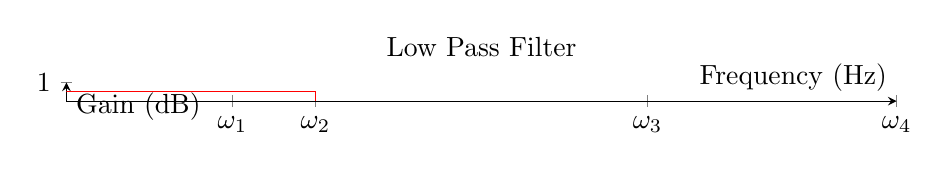
\begin{tikzpicture}
    \begin{axis}[
        xlabel={Frequency (Hz)},
        ylabel={Gain (dB)},
        title={Low Pass Filter},
        width=\linewidth,
        height=0.15\linewidth,
        xmin=0, xmax=10,
        ymin=0, ymax=1,
        ytick={1},
        xtick={0, 2, 3, 7, 10},
        xticklabels={0, $\omega_1$, $\omega_2$, $\omega_3$, $\omega_4$, $\omega_5$},
        axis lines=middle,
    ]
    \addplot[domain=0:10, samples=100, color=red] coordinates {
        (0, 0.5)
        (3, 0.5)
        (3, 0)
    };
    \end{axis}
\end{tikzpicture}
                        \caption{Low Pass Filter}
                    \end{figure}
                    \begin{figure}[H]
                        \centering
                        \begin{circuitikz}[american]
                            \draw (0,0) to[voltage source, v=$v_i\left(\omega\right)$, invert] (0,2);
                            \draw (0,2) to[short] (2,2);
                            \draw (2,2) to[resistor, l^=$1\text{k}\Omega$] (4,2);
                            \draw (4,2) to[capacitor, l^=$1\mu $F] (4,0);
                            \draw (4,0) to[short] (0,0);
                            \draw (4,2) to[short] (6,2);
                            \draw (4,0) to[short] (6,0);
                            \draw (6,1) node[right] {$v_o\left(\omega\right)$};
                            \draw[dotted] (2,-1) rectangle (5.5,3);
                        \end{circuitikz}
                    \end{figure}
                    \begin{align*}
                        v_o(\Omega) &= \frac{\frac{1}{j\omega C}}{R + \frac{1}{j\omega C}}v_i(\omega)\\
                        \frac{v_0 (\omega)}{v_i (\omega)} &= \frac{1}{j\omega RC + 1}\\
                        \intertext{For $R = 1\text{k}\Omega$ and $C = 1\mu F$}
                        H(\omega) &= \frac{1000}{j\omega + 1000}\\
                        H(62.8) \approx 1 && H(62800) = 0.016 \angle -89^{\circ}
                    \end{align*}
                    \subsubsection{Plotting the Response}
                        \begin{figure}[H]
                            \centering
                            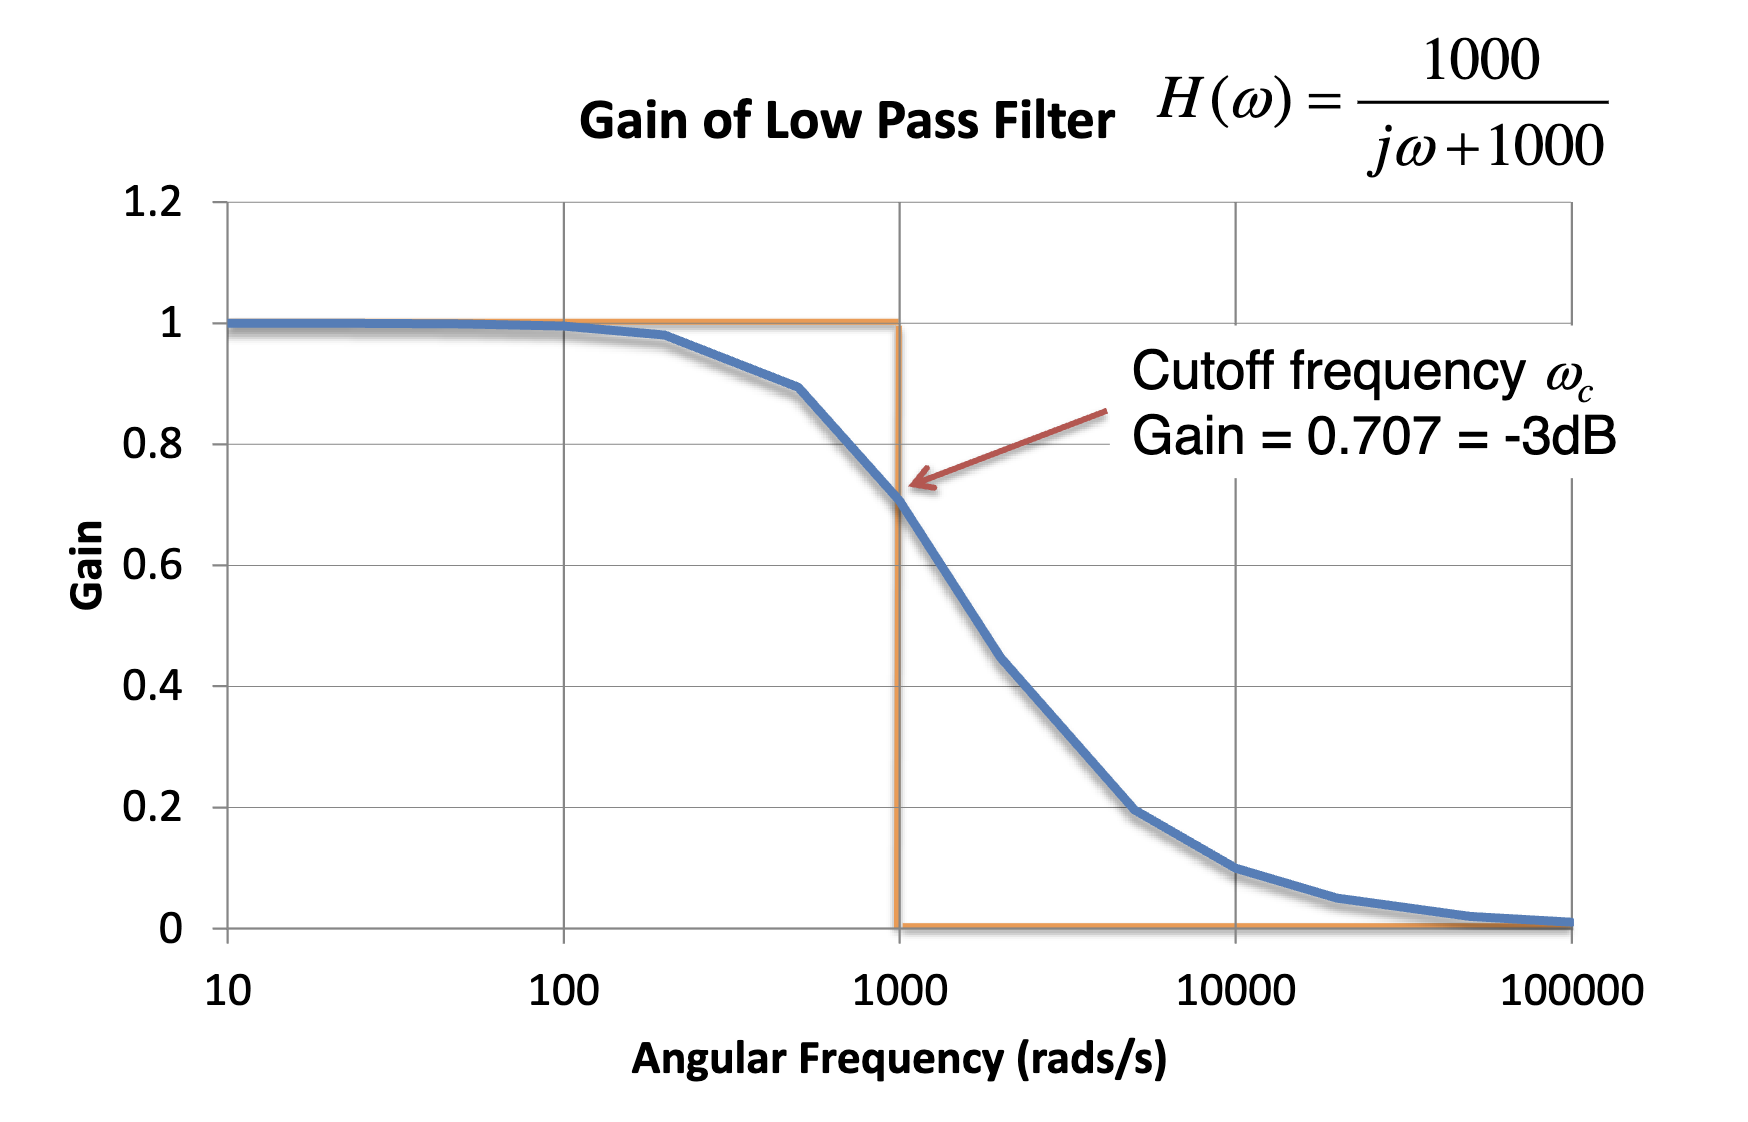
\includegraphics[width=0.5\linewidth]{figures/lowpass_bode.png}
                            \caption{Low Pass Filter Bode Plot}
                        \end{figure}
                    \subsubsection{Desigining a Low Pass Filter}
                        Find the required \textbf{cutoff frequency} $\omega_c$ in radians per second (remember $\omega_c = 2\pi f$)\\
                        Choose a value for $R$ and calculate $C$ such that $\omega_c = \frac{1}{RC}$\\
                        \begin{minipage}{0.5\linewidth}
                            \begin{figure}[H]
                                \centering
                                \begin{circuitikz}[american]
                                    \draw (0,0) to[voltage source, v=$v_i\left(\omega\right)$, invert] (0,2);
                                    \draw (0,2) to[short] (2,2);
                                    \draw (2,2) to[resistor, l^=R] (4,2);
                                    \draw (4,2) to[capacitor, l^=C] (4,0);
                                    \draw (4,0) to[short] (0,0);
                                    \draw (4,2) to[short] (6,2);
                                    \draw (4,0) to[short] (6,0);
                                    \draw (6,1) node[right] {$v_o\left(\omega\right)$};
                                    \draw[dotted] (2,-1) rectangle (5.5,3);
                                \end{circuitikz}
                            \end{figure}
                        \end{minipage}
                        \begin{minipage}{0.5\linewidth}
                            \begin{align*}
                                H(\omega) &= \frac{\frac{1}{RC}}{j\omega + \frac{1}{RC}}\\
                                \omega_c &= \frac{1}{RC}
                            \end{align*} 
                        \end{minipage}
                \subsection{High Pass Filter}
                    Similar to a low pass filter, but the capacitor and resistor are swapped\\
                    \subsubsection{Desigining a High Pass Filter}
                        \begin{minipage}{0.5\linewidth}
                            \begin{figure}[H]
                                \centering
                                \begin{circuitikz}[american]
                                    \draw (0,0) to[voltage source, v=$v_i\left(\omega\right)$, invert] (0,2);
                                    \draw (0,2) to[short] (2,2);
                                    \draw (2,2) to[capacitor, l^=C] (4,2);
                                    \draw (4,2) to[resistor, l^=R] (4,0);
                                    \draw (4,0) to[short] (0,0);
                                    \draw (4,2) to[short] (6,2);
                                    \draw (4,0) to[short] (6,0);
                                    \draw (6,1) node[right] {$v_o\left(\omega\right)$};
                                    \draw[dotted] (2,-1) rectangle (5.5,3);
                                \end{circuitikz}
                            \end{figure}
                        \end{minipage}
                        \begin{minipage}{0.5\linewidth}
                            \begin{align*}
                                v_o(\omega) &= \frac{R}{R + \frac{1}{j\omega C}}v_i(\omega)\\
                                \frac{v_0 (\omega)}{v_i (\omega)} = H(\omega) &= \frac{j\omega RC}{j\omega RC + 1}\\\\
                                \omega_c &= \frac{1}{RC}
                            \end{align*}
                        \end{minipage}
                    \subsubsection{Plotting the Response}
                        \begin{figure}[H]
                            \centering
                            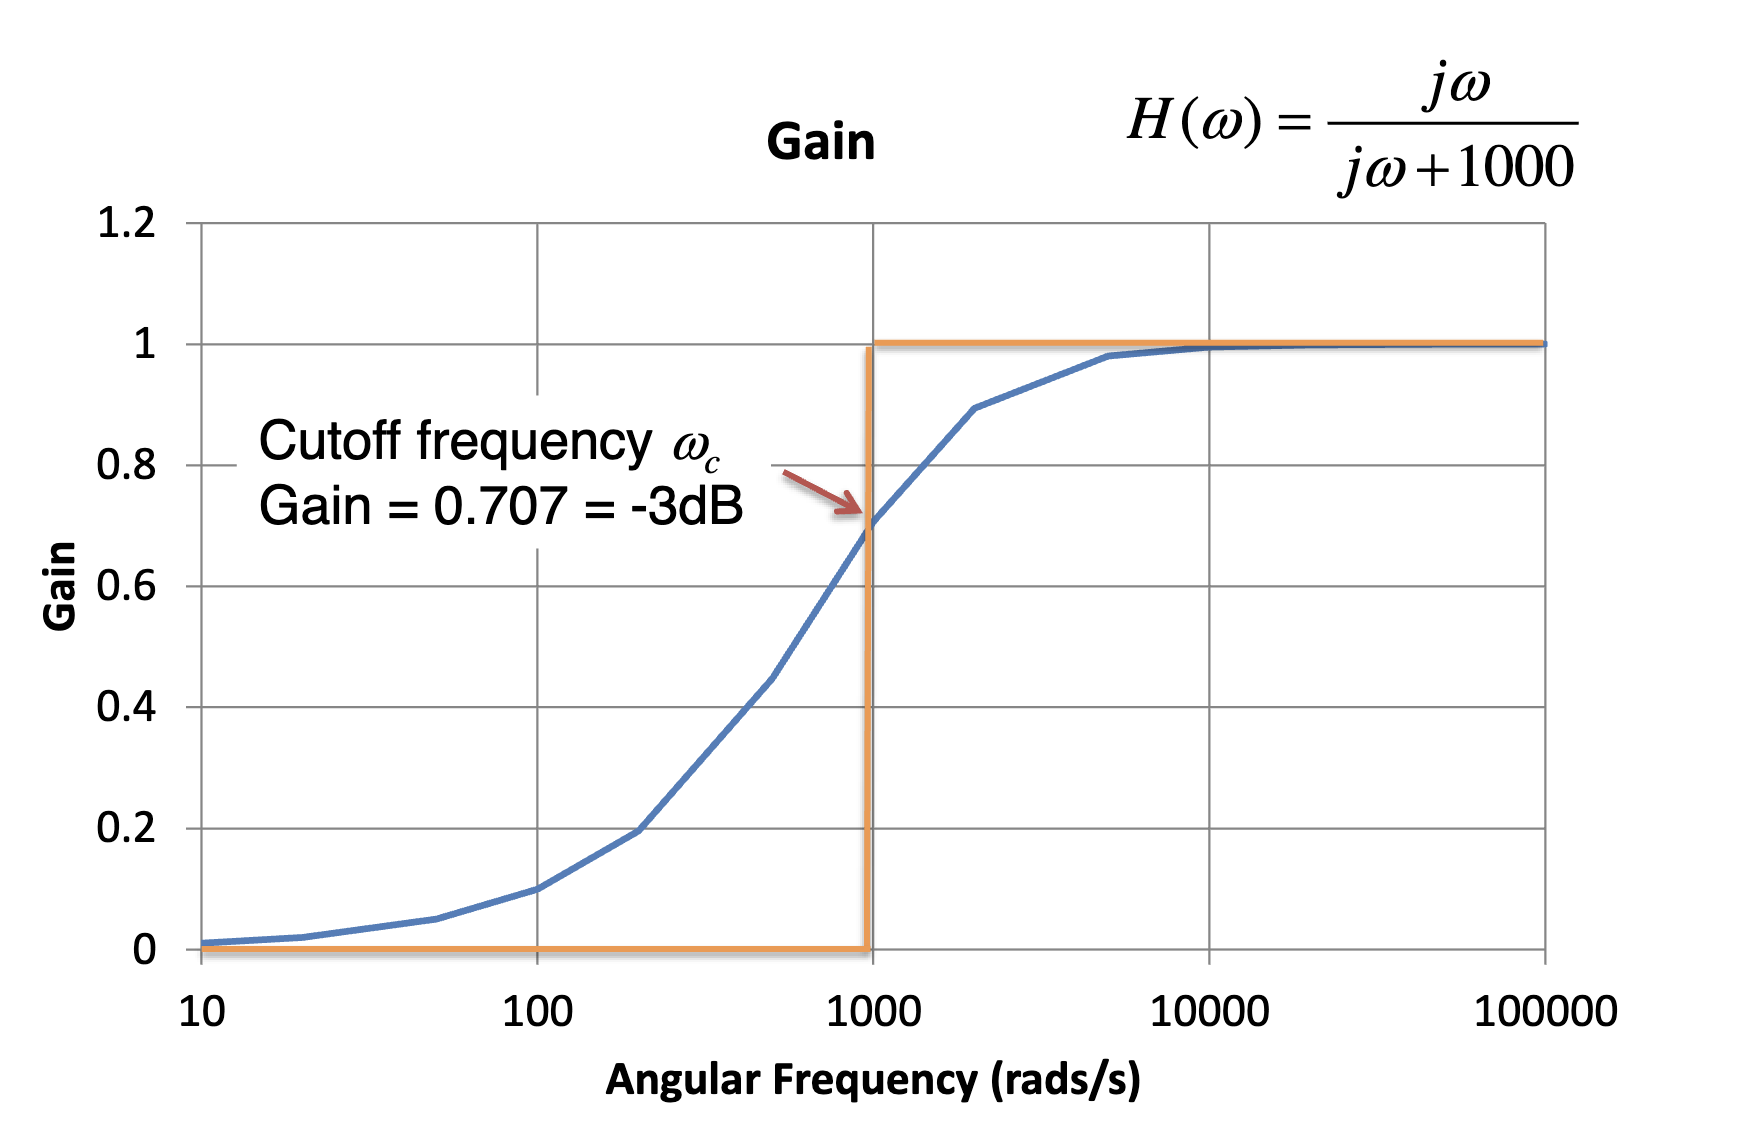
\includegraphics[width=0.5\linewidth]{figures/highpass_bode.png}
                            \caption{High Pass Filter Bode Plot}
                        \end{figure}
            \section{Active Filters}
                \subsection{Op-Amps}
                    \begin{figure}[H]
                        \begin{subfigure}{0.45\linewidth}
                            \centering
                            \begin{circuitikz}[american]
                                \draw (0,0) node[op amp] (opamp) {};
                                \node[above] at (-3,0.7) {$v_{in}$};
                                \draw (-3,0.5) to[resistor, R=$Z_1$] (opamp.-);
                                \draw (opamp.-) to[short] ++(0,1) to[short] ++(0.5,0) to[resistor, R=$Z_2$] ++(3,0) to[short] ++(0,-1.5);
                                \draw (opamp.out) to[short] ++(2,0) node[right] {$v_o$};
                                % ground
                                \draw (opamp.+) to[short] ++(-0.5,0) to[short] ++(0,-0.5) node[ground] {};
                            \end{circuitikz}
                            \subcaption{Inverting Amplifier}
                        \end{subfigure}
                        \begin{subfigure}{0.45\linewidth}
                            \centering
                            \begin{circuitikz}[american]
                                \draw (0,0) node[op amp, noinv input up] (opamp) {};
                                \node[above] at (-3,0.7) {$v_{in}$};
                                \draw (-3,0.5) to[short] (opamp.+);
                                \draw (opamp.-) to[short] ++(0,-1) to[resistor, R=$Z_1$] ++(-2,0) node[ground] {};
                                \draw (opamp.out) to[short] ++(0,-1.5) to[resistor, R=$Z_2$] ++(-2.38,0);
                                \draw (opamp.out) to[short] ++(2,0) node[right, R=$Z_3$] {$v_o$};
                            \end{circuitikz}
                            \subcaption{Non-Inverting Amplifier}
                        \end{subfigure}
                        \caption{Active Filters}
                    \end{figure}
                \subsection{Using an Op Amp}
                    \subsubsection{Active High Pass Filter}
                        \begin{minipage}{0.7\linewidth}
                            \begin{figure}[H]
                                \centering
                                \begin{circuitikz}[american]
                                    \draw (0,0) node[op amp] (opamp) {};
                                    \draw (-4.5, 0.5) to [capacitor, l_=$1\mu$F] ++(1.5,0);
                                    \node[above] at (-5,0.7) {$v_{in}$};
                                    \draw (-3,0.5) to[resistor, l=$1\text{k}\Omega$] (opamp.-);
                                    \draw (opamp.-) to[short] ++(0,1) to[short] ++(0.5,0) to[resistor, l=$10\text{k}\Omega$] ++(3,0) to[short] ++(0,-1.5);
                                    \draw (opamp.out) to[short] ++(2,0) node[right] {$v_o$};
                                    % ground
                                    \draw (opamp.+) to[short] ++(-0.5,0) to[short] ++(0,-0.5) node[ground] {};
                                    \draw[dotted, thick] (-4.5, -0.5) rectangle (-1.25, 1.5) node[above] at (-3.25, 1.5) {$Z_1$};
                                    \draw[dotted, thick] (-1, 1) rectangle (2.25, 2.5) node[above] at (0.625, 2.5) {$Z_2$};
                                \end{circuitikz}
                                \subcaption{Active High Pass Filter}
                            \end{figure}
                        \end{minipage}
                        \begin{minipage}{0.3\linewidth}
                            \begin{align*}
                                v_o &= -\frac{Z_2}{Z_1}v_{in}\\
                                \frac{v_o}{v_{in}} &= -\frac{R_2}{R_1 + \frac{1}{j\omega C_1}} = -\frac{R_2}{R_1} \frac{j\omega}{j\omega + \frac{1}{R_1 C_1}}\\
                            \end{align*}
                            High pass filter with\\
                            $\omega_c = \frac{1}{R_1 C_1} = \frac{1}{10^3 \times 10^{-6}} = 1000\text{rad/s}$\\\\
                            Gain of $-\frac{R_2}{R_1} = -10$ in passband
                        \end{minipage}
                    \subsubsection{Active Low Pass Filter}
                        \begin{minipage}{0.7\linewidth}
                            \begin{figure}[H]
                                \centering
                                \begin{circuitikz}[american]
                                    \draw (0,0) node[op amp] (opamp) {};
                                    \node[above] at (-3.5,0.7) {$v_{in}$};
                                    \draw (-3.5,0.5) to[resistor, R=1k$\Omega$] (opamp.-);
                                    \draw (opamp.-) to[short] ++(0,1) to[resistor, R=10k$\Omega$]++(3,0) to[short] ++(0,-1.5);
                                    \draw (opamp.-) to[short] ++(0,2.5) to[capacitor, C=$1\mu$F] ++(3,0) to[short] ++(0,-3);
                                    \draw (opamp.out) to[short] ++(2,0) node[right] {$v_o$};
                                    % ground
                                    \draw (opamp.+) to[short] ++(-0.5,0) to[short] ++(0,-0.5) node[ground] {};
                                    \draw[dotted, thick] (-3, 0) rectangle (-1.5, 1.5) node[above] at (-2.25, 1.5) {$Z_1$};
                                    \draw[dotted, thick] (-0.5, 1) rectangle (1, 4) node[above] at (0.25, 4) {$Z_2$};
                                \end{circuitikz}
                                \subcaption{Active Low Pass Filter}
                            \end{figure}
                        \end{minipage}
                        \begin{minipage}{0.3\linewidth}
                            \begin{align*}
                                v_o &= -\frac{Z_2}{Z_1}v_{in}\\
                                &= \frac{\frac{1}{\frac{1}{R_2} + j\omega C_2}}{R_1}v_{in}\\
                                \frac{v_o}{v_{in}} = H(\omega) &= -\frac{R_2}{R_1} \frac{1}{1+j\omega R_2C_2}\\
                                &= -\frac{R_2}{R_1} \frac{\frac{1}{R_2C_2}}{j\omega + \frac{1}{R_2C_2}}\\
                            \end{align*}
                            Low pass filter with \\$\omega_c = \frac{1}{R_2 C} = \frac{1}{10^4 \times 10^{-6}} = 100\text{rad/s}$\\\\
                            Gain of $-\frac{R_2}{R_1} = -10$ in passband
                        \end{minipage}
            \section{Band Pass and Band Stop Filters}
                \begin{figure}[H]
                    \centering
                    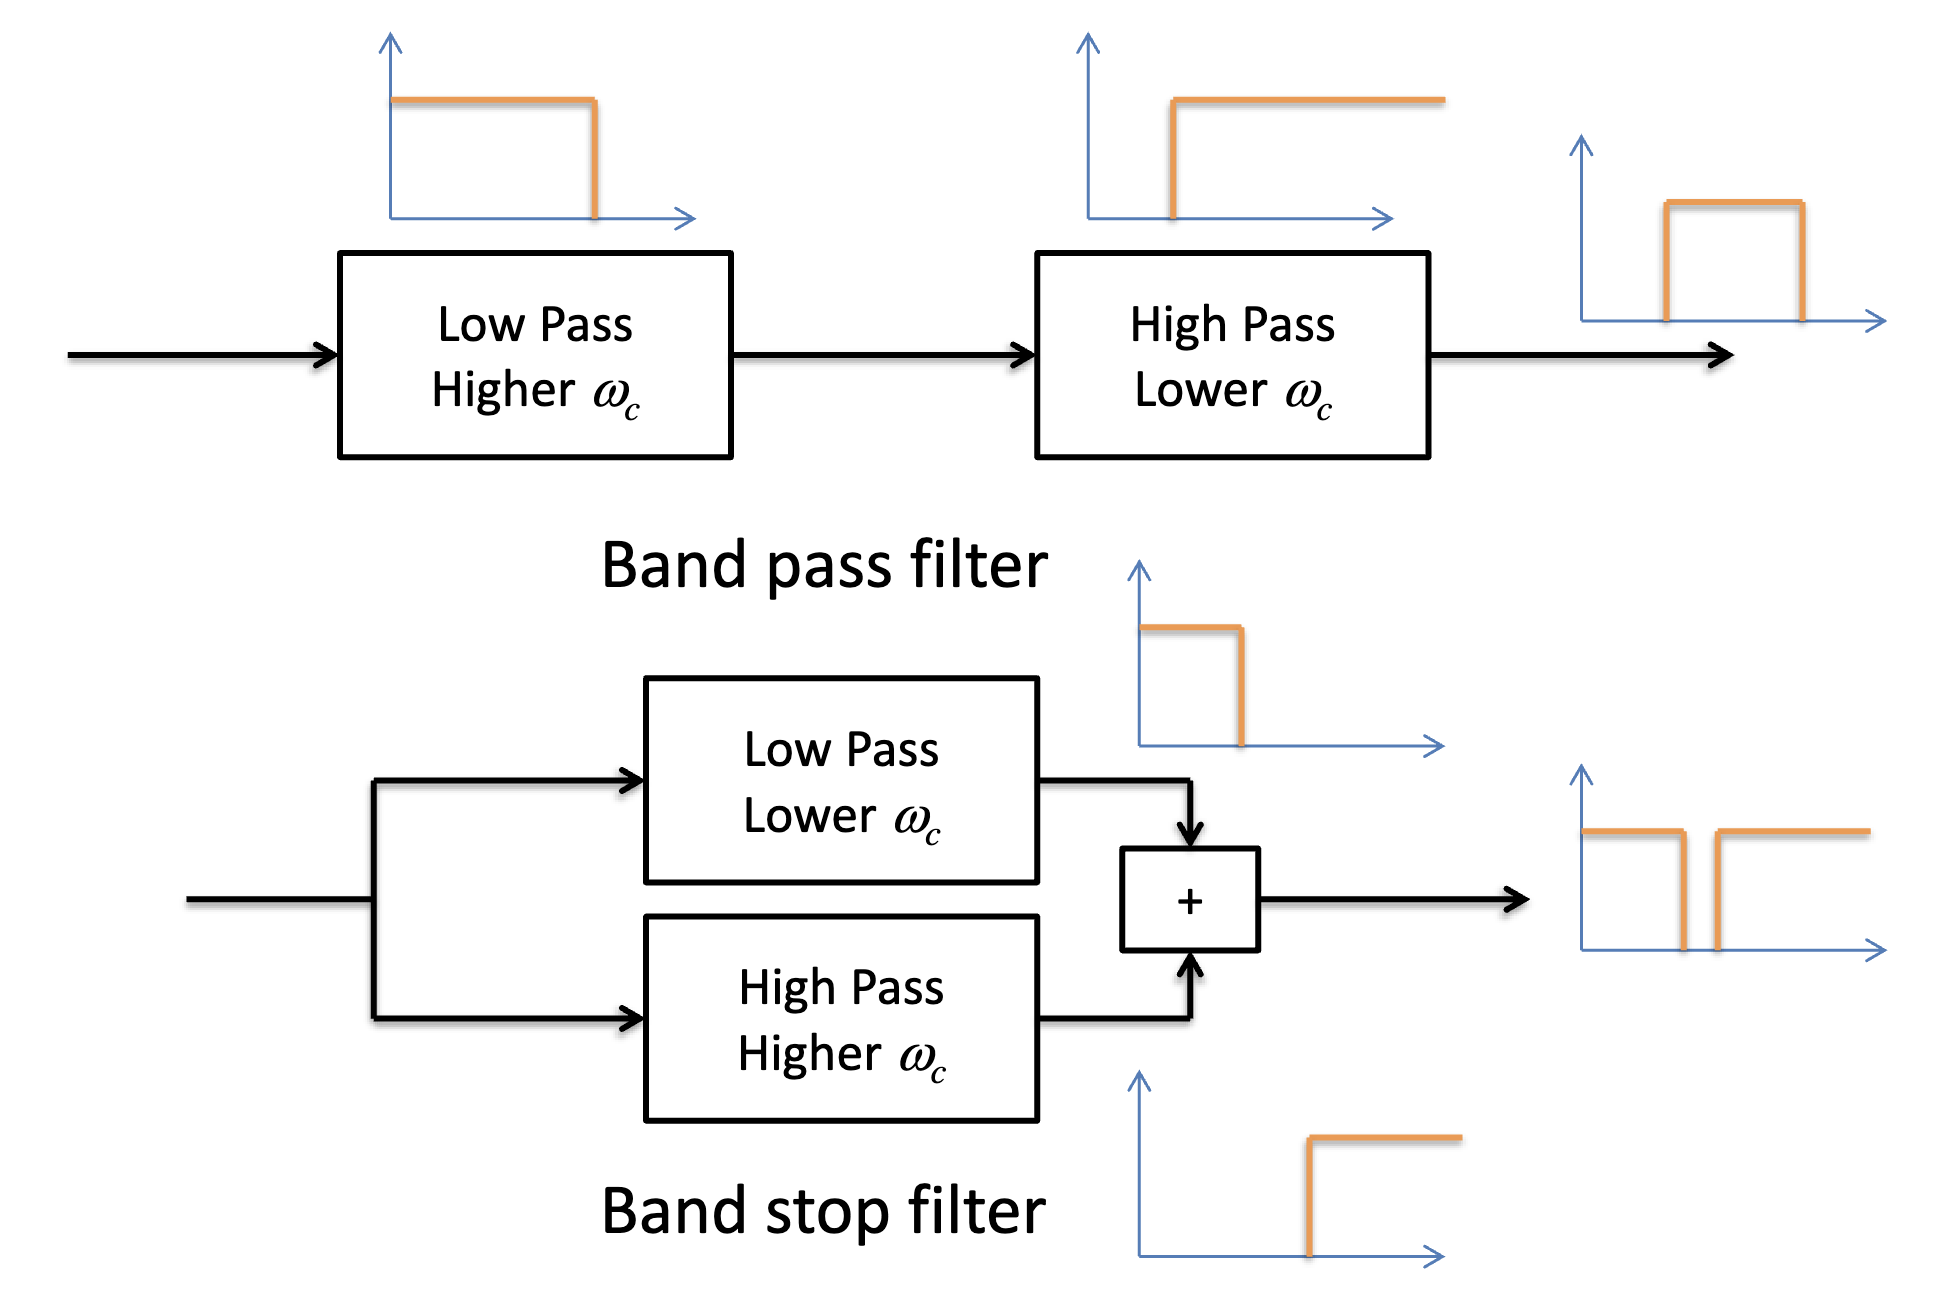
\includegraphics[width=0.6\linewidth]{figures/band_pass_stop.png}
                    \caption{Band Pass and Band Stop Filters}
                \end{figure}
        \chapter{Tutorials}
            \section{Tutorial 7 \- Sequential Switching}
Consider the circuit below. The initial current in the inductor is $i_l(0-) = 0$. Find expressions for
$iL(t)$ and $v(t)$ for $t \geq 0$ and sketch to scale versus time.
\begin{figure}[H]
    \centering
    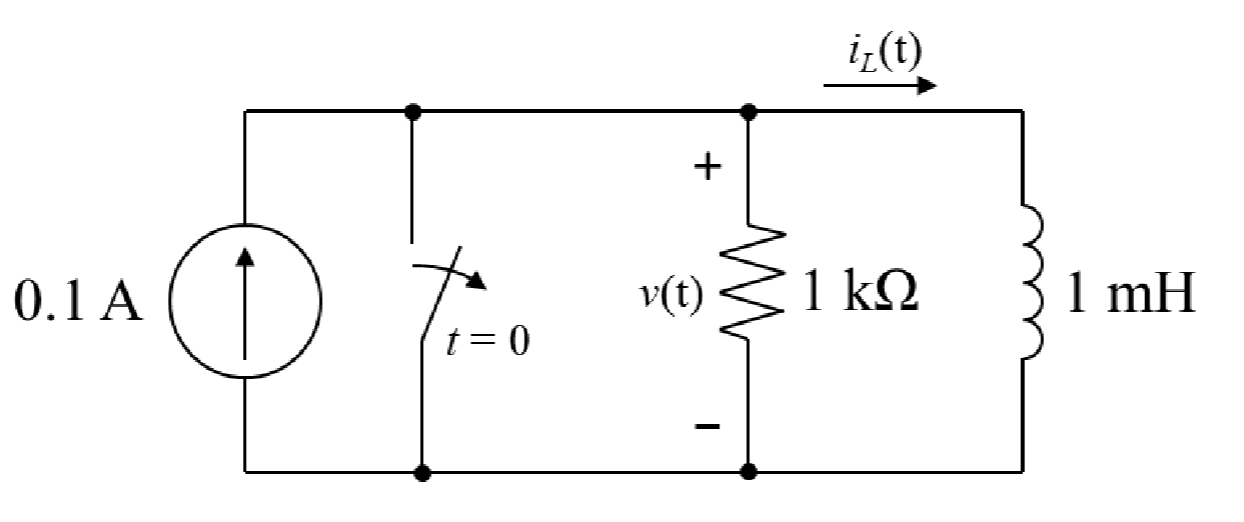
\includegraphics[width=0.4\linewidth]{tutorials/figures/seq_switch_practice.png}
\end{figure}
The given circuit is an RL circuit, therefore, step response is given by
\begin{equation*}
    i(t) = \frac{V_s}{R} + \left(I_0 - \frac{V_s}{R}\right)e^{-\frac{R}{L}t}
\end{equation*}
By applying a source transformation (Norton equivalent to Thevenin equivalent) we get
\begin{align*}
    V_s &= I_s R = 0.1 \times 1 \times 10^3 = 0.1 \times 10^3 V = 100V\\
\end{align*}
Using this we get that
\begin{align*}
    i(t) &= \frac{100}{1000} + \left(0 - \frac{100}{1000}\right)e^{-\frac{1000}{1\times{-3}}t} &&= 0.1 - 0.1e^{-1\times10^6 t} \\
    v(t) &= L \odv{i}{t} = 1\times10^{-3} \times \odv{}{t} \left(0.1 - 0.1e^{-1\times10^6 t}\right) = 0.1\times10^3 e^{-1\times10^6 t} &&= 100e^{-1\times10^6 t}
\end{align*}
\subsection{Tutorial Question}
    Igor the Mad Scientist is planning to reanimate a corpse (again). His plan is to capture energy
    from a lightning bolt into a capacitor, and then to discharge the capacitor into the torso and
    brain. The lower body is reanimated from a voltage supply. The electrical models of the body
    parts are shown in the figure below
    \begin{figure}[H]
        \centering
        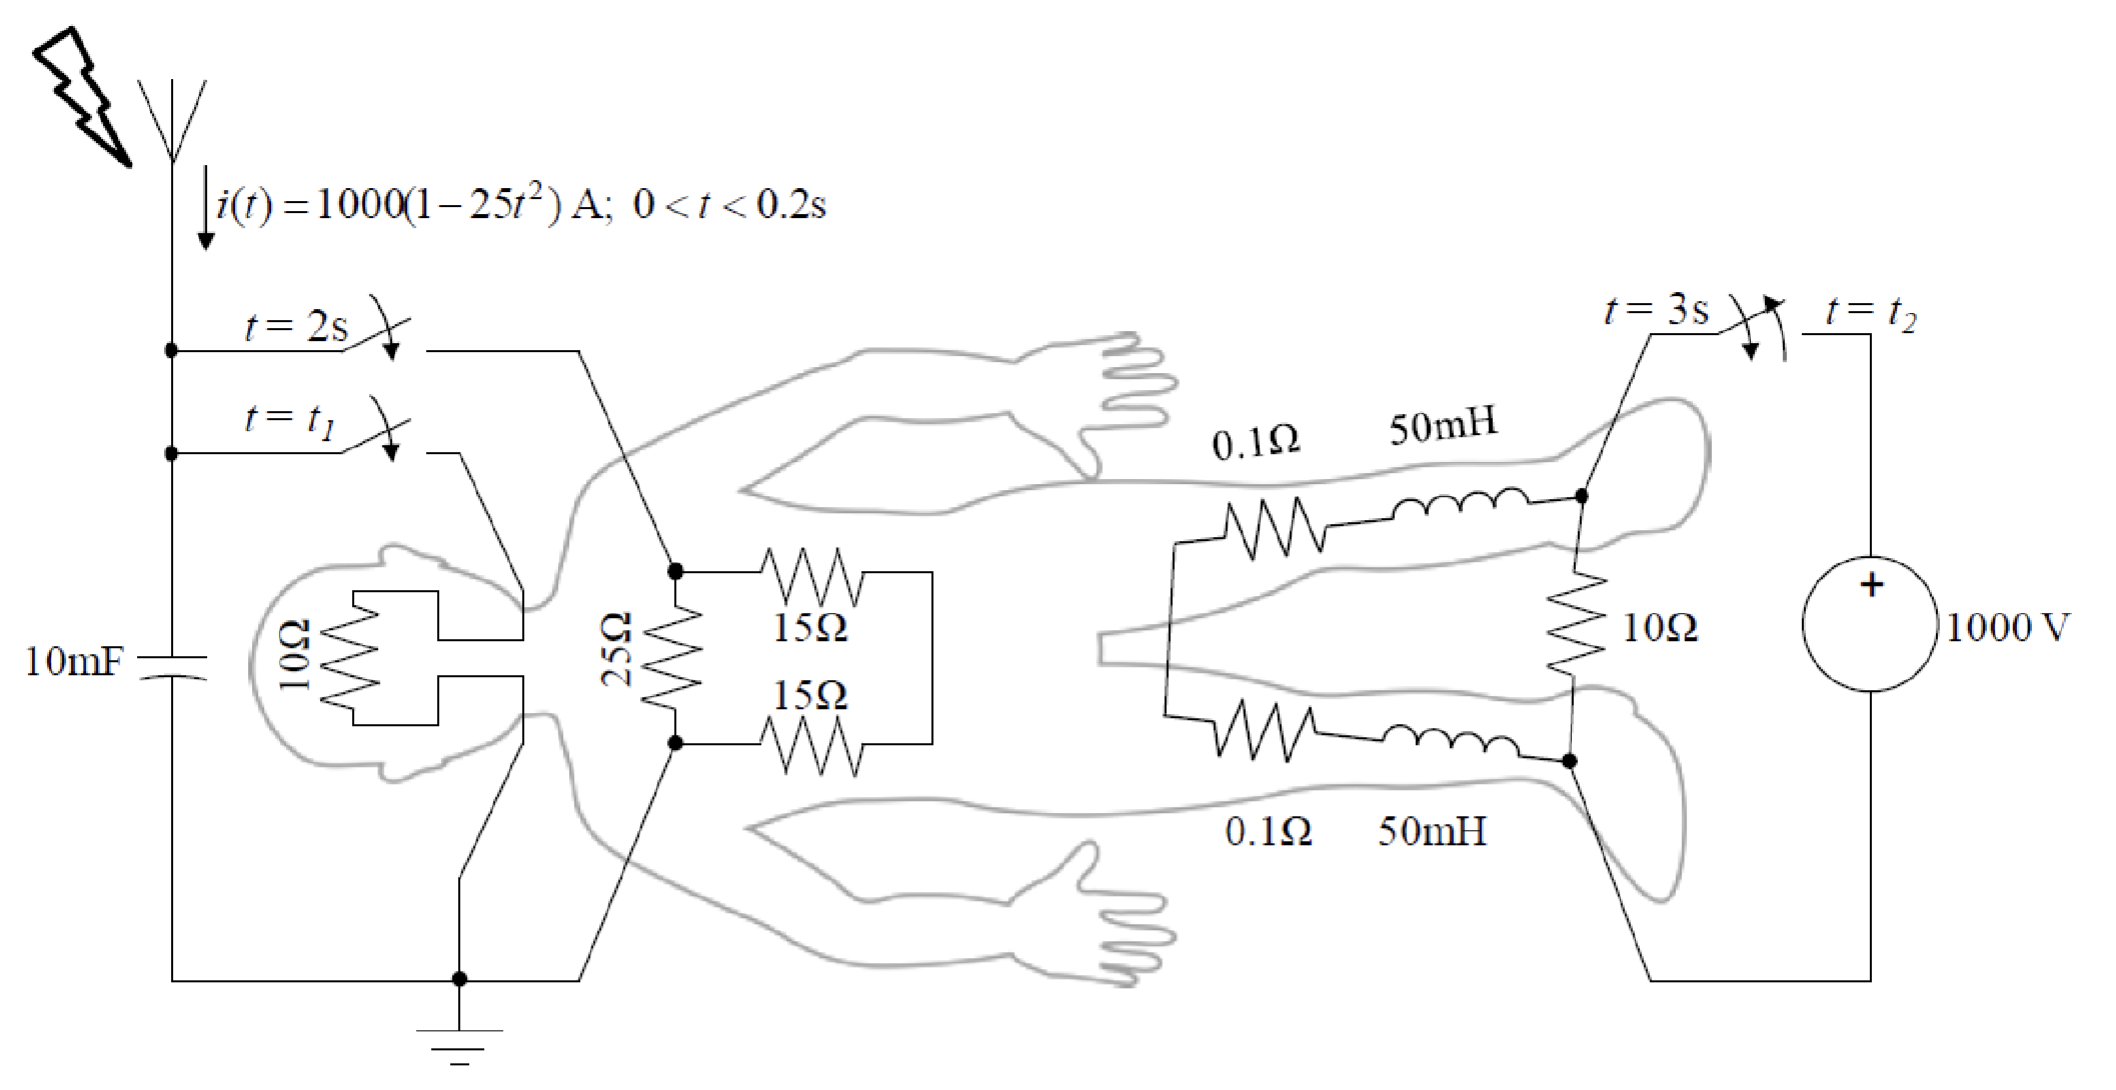
\includegraphics[width=0.6\linewidth]{tutorials/figures/frankenstein.png}
    \end{figure}
    The steps for corpse re-animation are as follows:
    \begin{itemize}
        \item \textbf{Step 1}: Capture a lightning strike into a discharged capacitor. The moment of the lightning
        strike marks $t = 0$. The lightning strike has a duration of 200 ms, and creates a current $i(t) =
        1000(1 - 25t^2)$ A for $0 < t < 0.2s$.
        \item \textbf{Step 2}: At t = 2s, start discharging the capacitor across the torso.
        \item \textbf{Step 3}: When the capacitor voltage falls to 1000 V, close the switch to discharge the capacitor
        into the brain (through the neck bolts).
        \item \textbf{Step 4}: At t = 3s, close the switch to connect the legs to the 1000 V source.
        \item \textbf{Step 5}: When the current reaches 500A, open the switch to disconnect the legs from the 1000 V
        source.
        \item \textbf{Step 6}: Once the leg current drops below 50 mA, and the capacitor voltage drops below 10 V
        the corpse will come to life. Disconnect the cables and feed your new monster some tea and
        cake.
    \end{itemize}
    Igor is using computer controlled switching for precise timing. He needs your help to work out
    the right time for critical switching activities.
    \begin{enumerate}
        \item Find the voltage of the capacitor after the lightning strike for $0.2 < t < 2s$.\\
        By isolating the circuit for the step response we get
        % minipage 1
        \begin{figure}[H]
            \centering
            \begin{circuitikz}[american]
                \draw
                (-1,5) to[capacitor, C=100mF] ++(0,-2.5)
                (-1,5) to[short] ++(2,0)
                (1,5) to[resistor, R=10$\Omega$] ++(0,-2.5)
                (-1,2.5) to[short] ++(2,0);
                \draw (-1,6) to[short, i=$i(t)$, invert] (-1,5);
            \end{circuitikz}
        \end{figure}
        As this is an RC Circuit\\
        \begin{minipage}{0.45\textwidth}
            \begin{flalign*}
                V(t) &= \frac{1}{C} \int^{t}_{0} i(\tau) + v(0) \, d\tau \\
                &= \frac{1}{10^{10^{-3}}} \int^{t}_{0} 1000(1 - 25\tau^2) \, d\tau + 0 \\
                &= 10^5 \left(\tau - \frac{25}{3}\tau^3\right) \Big|^{t}_{0} \\
                &= 10^5 \left(t - \frac{25}{3}t^3\right)
            \end{flalign*}
        \end{minipage}
        \begin{minipage}{0.45\textwidth}
            \begin{flalign*}
                V(0.2) &= 10^5 \left(0.2 - \frac{25}{3}(0.2)^3\right) \\
                &= 10^5 \left(0.2 - \frac{25}{3}(0.008)\right) \\
                &= 10^5 \left(0.2 - 0.066\right) \\
                &= 10^5 \times 0.13\overline{3}\,\text{V} \\
                &= 13.33\overline{3}\,\text{kV}
            \end{flalign*}
        \end{minipage}
        \item Find an expression for the capacitor voltage while the capacitor is discharging into the
        torso only. When will the capacitor be sufficiently discharged to connect the capacitor to
        the brain?\\
        Capacitor will start discharging at $t=2s$ and will be sufficiently discharged when $V(t) = 1000V$\\
        Find the circuit at $t=2s$
        \begin{figure}[H]
            \centering
            \begin{circuitikz}[american]
                \draw
                (-1,5.5) to[capacitor, l_=$10$mF] ++(0,-2)
                (-1,3.5) to[short] ++(1.5,0)
                (0.5,3.5) to[resistor, R=$25\Omega$] ++(0,2)
                (-1,5.5) to[short] ++(1.5,0)
                to[resistor, R=$15\Omega$] ++(1.5,0)
                (2,5.5) to[short] ++(0,-2)
                (0.5,3.5) to[resistor, R=$15\Omega$] ++(1.5,0);
            \end{circuitikz}
        \end{figure}
        Note that the two $15\Omega$ resistors are in series, therefore, we can replace them with a single $30\Omega$ resistor.\\
        This $30\Omega$ resistor is in parallel with the $25\Omega$ resistor, therefore, we can replace them with a single $\left(\frac{1}{30} + \frac{1}{25}\right)^{-1} = \frac{150}{11}\Omega$ resistor.\\
        This gives the following circuit
        \begin{figure}[H]
            \centering
            \begin{circuitikz}[american]
                \draw
                (-1,5.5) to[capacitor, l_=$10$mF] ++(0,-2)
                (-1,3.5) to[short] ++(1.5,0)
                (0.5,3.5) to[resistor, l_=$\frac{150}{11}\Omega$] ++(0,2)
                (-1,5.5) to[short] ++(1.5,0);
            \end{circuitikz}
        \end{figure}
        Using this RC circuit we can solve for when voltage is 1000, where $v(0) = 13.33\overline{3}\,\text{kV}$
        \begin{flalign*}
            v(t) &= v(0)e^{-\frac{t}{RC}}\\
            1000 &= 13.33\overline{3}e^{-\frac{t}{\frac{150}{11} \times 10^{-3}}}\\
            \intertext{Using calculator}
            t &= 0.3532s
        \end{flalign*}
        Noting that this time is relative to the 2 seconds since the lightning strike, therefore, the time since the lightning strike is $t=2.3532s$
        \item When will the capacitor voltage fall below 10V?
        First, include the head that is now connected
        \begin{figure}[H]
            \centering
            \begin{circuitikz}[american]
                \draw
                (-1,5.5) to[capacitor, l_=$10$mF] ++(0,-2)
                (-1,3.5) to[short] ++(1.5,0)
                (0.5,3.5) to[resistor, l_=$10\Omega$] ++(0,2)
                (-1,5.5) to[short] ++(1.5,0)
                to[short] ++(1.5,0)
                (2,5.5) to[resistor, l=$\frac{150}{11}\Omega$] ++(0,-2)
                (0.5,3.5) to[short] ++(1.5,0);
            \end{circuitikz}
        \end{figure}
        Note that the two resistors are in parallel therefore we can replace them with a single $\left(\frac{1}{10} + \frac{1}{\frac{150}{11}}\right)^{-1} = 5.77\Omega$ resistor.\\
        This gives the following circuit
        \begin{figure}[H]
            \centering
            \begin{circuitikz}[american]
                \draw
                (-1,5.5) to[capacitor, l_=$10$mF] ++(0,-2)
                (-1,3.5) to[short] ++(1.5,0)
                (0.5,3.5) to[resistor, l_=$5.77\Omega$] ++(0,2)
                (-1,5.5) to[short] ++(1.5,0);
            \end{circuitikz}
        \end{figure}
        Using this RC circuit we can solve for when voltage is 10, where $v(0) = 1000\,\text{V}$\
        \begin{flalign*}
            v(t) &= v(0)e^{-\frac{t}{RC}}\\
            10 &= 1000e^{-\frac{t}{5.77 \times 10^{-3}}}\\
            \intertext{Using calculator}
            t &= 0.2657s
        \end{flalign*}
        As this time is relative to the time from part 3, the time since the lightning strike is $t=2.6189s$ 
        \item Find an expression for the leg current when the voltage source is connected to the legs.
        When should the switch connecting the voltage source to the legs be opened?\\
        Looking at the torso circuit we see the following
        \begin{figure}[H]
            \centering
            \begin{circuitikz}[american]
                \draw
                (4,3) to[short] ++(1.5,0)
                to[voltage source, invert, l_=$1000V$] ++(0,2)
                (1,5) to[short] ++(0,-2)
                to[resistor, l=$0.1\Omega$] ++(1.5,0)
                to[inductor, l=50mH] ++(1.5,0)
                to[resistor, l=$10\Omega$] ++(0,2)
                (1,5) to[resistor, l=$0.1\Omega$] ++(1.5,0)
                to[inductor, l=50mH] ++(1.5,0)
                (4,5) to[short] ++(1.5,0);
            \end{circuitikz}
        \end{figure}
        Noting that the two $0.1\Omega$ resistors are in series, we can combine them into a single $0.2\Omega$ resistor.\\
        Noting that the two $50$mH inductors are in series, we can combine them into a single $100$mH inductor.\\
        This gives the following circuit
        \begin{figure}[H]
            \centering
            \begin{circuitikz}[american]
                \draw
                (4,3) to[short] ++(1.5,0)
                to[voltage source, invert, l_=$1000V$] ++(0,2)
                (4,3) to[resistor, l=$10\Omega$] ++(0,2)
                (4,3) to[short] ++(-3,0)
                to[short] ++(0,2)
                to[resistor, l=$0.2\Omega$] ++(1.5,0)
                to[inductor, l=$100$mH] ++(1.5,0)
                (4,5) to[short] ++(1.5,0);
            \end{circuitikz}
        \end{figure}
        Noting that the $0.2\Omega$ resistor and $10\Omega$ resistor are in parallel, we can combine them into a single $\left(\frac{1}{0.2} + \frac{1}{10}\right)^{-1} = 0.196\Omega$ resistor.\\
        This gives the following circuit
        \begin{figure}[H]
            \centering
            \begin{circuitikz}[american]
                \draw
                (2.5,5) to[resistor, l=$0.196\Omega$] ++(0,-2)
                to[short] ++(1.5,0)
                to[short] ++(1.5,0)
                to[voltage source, invert, l_=$1000V$] ++(0,2)
                (2.5,5) to[inductor, l=100mH] ++(3,0);
            \end{circuitikz}
        \end{figure}
        \begin{flalign*}
            i(t) &= \frac{V_s}{R} + \left(I_0 - \frac{V_s}{R}\right)e^{-\frac{R}{L}t} \\
            &= \frac{1000}{0.196} + \left(0 - \frac{1000}{0.196}\right)e^{-\frac{0.196}{100\times10^{-3}}t} \\
            &= 5102.04 - 5102.04e^{-1.96t}\\
            v(t) &= L\odv{i}{t}\\
            &= 100\times10^{-3} \times \odv{}{t} \left(5102.04 - 5102.04e^{-1.96t}\right)\\
            &= 100\times10^{-3} \times 5102.04 \times 1.96e^{-1.96t}\\
            &= 100007e^{-1.96t}
            \intertext{When current is 500A, open the switch to disconnect legs}
            500 &= 5102.04 - 5102.04e^{-1.96t}\\
            \intertext{Using calculator}
            t &= 0.05262s \tag{Relative to 3 seconds}\\
            t_{\text{since lightning strike}} &= 3.05262s
        \end{flalign*}
        \item When will the leg current fall below 50mA?
        Now that the legs are disconnected, we get the following circuit
        \begin{figure}[H]
            \centering
            \begin{circuitikz}[american]
                \draw
                (1.5,5.5) to[resistor, l=$0.1\Omega$] ++(1.5,0)
                (3,5.5) to [inductor, l=50mH] ++(1.5,0)
                (4.5,5.5) to[resistor, l=$10\Omega$] ++(0,-1.5)
                (1.5,5.5) to[short] ++(0,-1.5)
                to[resistor, l=$0.1\Omega$] ++(1.5,0)
                (3,4) to [inductor, l=50mH] ++(1.5,0);
            \end{circuitikz}
        \end{figure}
        Noting that the two $0.1\Omega$ resistors are in series, we can combine them into a single $0.2\Omega$ resistor.\\
        Noting that the two $50$mH inductors are in series, we can combine them into a single $100$mH inductor.\\
        This gives the following circuit
        \begin{figure}[H]
            \centering
            \begin{circuitikz}[american]
                \draw
                (1.5,5.5) to[resistor, l=$0.2\Omega$] ++(1.5,0)
                (3,5.5) to [inductor, l=100mH] ++(1.5,0)
                (4.5,5.5) to[resistor, l=$10\Omega$] ++(0,-1.5)
                (1.5,5.5) to[short] ++(0,-1.5)
                to[short] ++(1.5,0)
                (3,4) to [short] ++(1.5,0);
            \end{circuitikz}
        \end{figure}
        Noting that the $0.2\Omega$ resistor and $10\Omega$ resistor are in series, we can combine them into a single $10.2\Omega$ resistor.\\
        This gives the following circuit
        \begin{figure}[H]
            \centering
            \begin{circuitikz}[american]
                \draw
                (1.5,5.5) to[resistor, l=$10.2\Omega$] ++(1.5,0)
                (3,5.5) to [inductor, l=50mH] ++(1.5,0)
                (4.5,5.5) to[short] ++(0,-1.5)
                (1.5,5.5) to[short] ++(0,-1.5)
                to[short] ++(1.5,0)
                (3,4) to [short] ++(1.5,0);
            \end{circuitikz}
        \end{figure}
        Natural response of an RL circuit
        \begin{flalign*}
            i(t) &= i(0)e^{-\frac{t}{R_2 C}}\\
            &= 500e^{-\frac{t}{10.2 \times 10^{-3}}}\\
            \intertext{When current is 50mA, open the switch to disconnect legs}
            0.05 &= 500e^{-\frac{t}{10.2 \times 10^{-3}}}\\
            \intertext{Using calculator}
            t &= 0.0903s \tag{Relative to $t_{\text{since lightning strike}}$ from 4}\\
            t_{\text{since lightning strike}} &= 3.14292s
        \end{flalign*}
    \end{enumerate}
\end{document}